%%%%%%%%%%%%%%%%%%%%%%%%%%%%%%%%%%%%%%%%%
% University Assignment Title Page 
% LaTeX Template
% Version 1.0 (27/12/12)
%
% This template has been downloaded from:
% http://www.LaTeXTemplates.com
%
% Original author:
% WikiBooks (http://en.wikibooks.org/wiki/LaTeX/Title_Creation)
%
% License:
% CC BY-NC-SA 3.0 (http://creativecommons.org/licenses/by-nc-sa/3.0/)
%
%%%%%%%%%%%%%%%%%%%%%%%%%%%%%%%%%%%%%%%%%
%\title{Title page with logo}
%----------------------------------------------------------------------------------------
%	PACKAGES AND OTHER DOCUMENT CONFIGURATIONS
%----------------------------------------------------------------------------------------

\documentclass[12pt]{article}
\usepackage[english]{babel}
\usepackage[utf8]{inputenc}
\usepackage{natbib}
\usepackage{amsmath}
\usepackage{color}
\usepackage[explicit]{titlesec}
\usepackage[hyphens,spaces,obeyspaces]{url}
\usepackage{graphicx}
\usepackage{caption}
\usepackage{subcaption}
\usepackage{grffile}
\usepackage{listings}

\lstset{language=python,keywordstyle={\bfseries \color{blue}}}


\begin{document}

\begin{titlepage}

\newcommand{\HRule}{\rule{\linewidth}{0.5mm}} % Defines a new command for the horizontal lines, change thickness here

\center % Center everything on the page
 
%----------------------------------------------------------------------------------------
%	HEADING SECTIONS
%----------------------------------------------------------------------------------------

\textsc{\LARGE University of St Andrews}\\[1.5cm] % Name of your university/college
\textsc{\Large Machine Learning}\\[0.5cm] % Major heading such as course name
\textsc{\large CS5014}\\[0.5cm] % Minor heading such as course title

%----------------------------------------------------------------------------------------
%	TITLE SECTION
%----------------------------------------------------------------------------------------

\HRule \\[0.4cm]
{ \huge \bfseries Classification}\\[0.4cm] % Title of your document
\HRule \\[1.5cm]
 
%----------------------------------------------------------------------------------------
%	AUTHOR SECTION
%----------------------------------------------------------------------------------------


\Large \emph{Author:}\\
 \textsc{150008022}\\[1cm] % Your name
 
%----------------------------------------------------------------------------------------
%	DATE SECTION
%----------------------------------------------------------------------------------------

{\large \today}\\[2cm] % Date, change the \today to a set date if you want to be precise

%----------------------------------------------------------------------------------------
%	LOGO SECTION
%---------------------------------------------------------------------------------------


\includegraphics[width = 4cm]{images/standrewslogo.png}
 
%----------------------------------------------------------------------------------------

\vfill % Fill the rest of the page with whitespace

\end{titlepage}

\subsection*{Goal}

The goal of this practical is to analyse a dataset in order to produce a classification model that can make predictions based on a set of inputs.

\tableofcontents

\pagebreak
\pagenumbering{arabic}
\setcounter{page}{1} 

\section{Loading Data}

To load the data, the paths to the relevant files are supplied as arguments to the \emph{\_\_main\_\_.py} script. The \emph{pandas} module was used to load the file contents into \emph{DataFrames}.

A test set was isolated from the original data using an 80\%-20\% split. Stratification was used to ensure that all classes were represented in the training data. 

% Merge data sets?

\section{Cleaning Data}

When originally loading the CSV files the parameter to raise an exception on missing or extra columns was included, and so it could be assumed that all rows had the same number of columns. The \lstinline{dtype=float} argument was also passed when loading the data to ensure that each column contained the expected numerical data. Any rows containing empty or \lstinline{NaN} values were dropped from the dataset.

\section{Data Visualisation and Analysis}

The input CSV was understood to have the structure shown in figure \ref{fig:structure}. Each value is either the mean, minimum, or maximum reading from 100 radar pulses, and these values are referred to as components.

\begin{figure}[!ht]
	\centering
	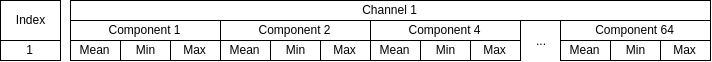
\includegraphics[width=\linewidth]{images/structure}
	\caption{The structure of each row of the CSV file which is repeated for minimum and maximum values.}
	\label{fig:structure}
\end{figure}

The mean, min, and max values were plotted for each channel for each sensor. The plots of the means of each channel for the book and plastic case objects are shown in figures \ref{fig:book} and \ref{fig:plasticcase} respectively. The difference between the resulting signals from the two objects are very clear.

\begin{figure}[!ht]
	\centering
	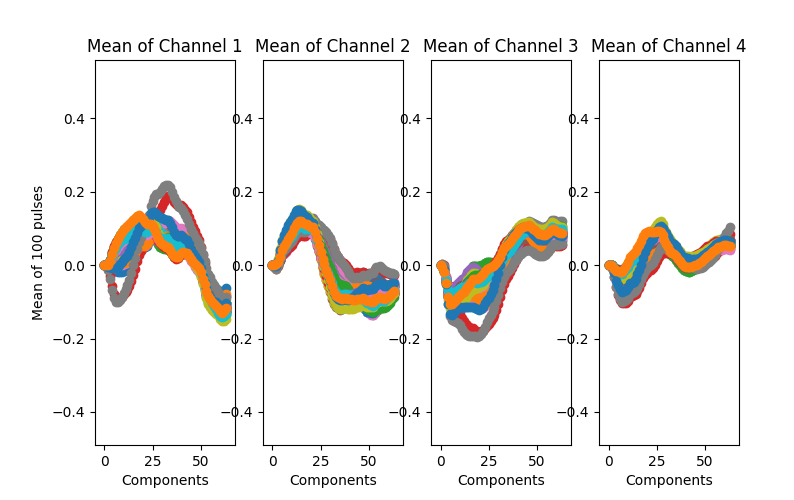
\includegraphics[width=\linewidth]{images/book}
	\caption{Mean of each channel measured for the book}
	\label{fig:book}
\end{figure}

\begin{figure}[!ht]
	\centering
	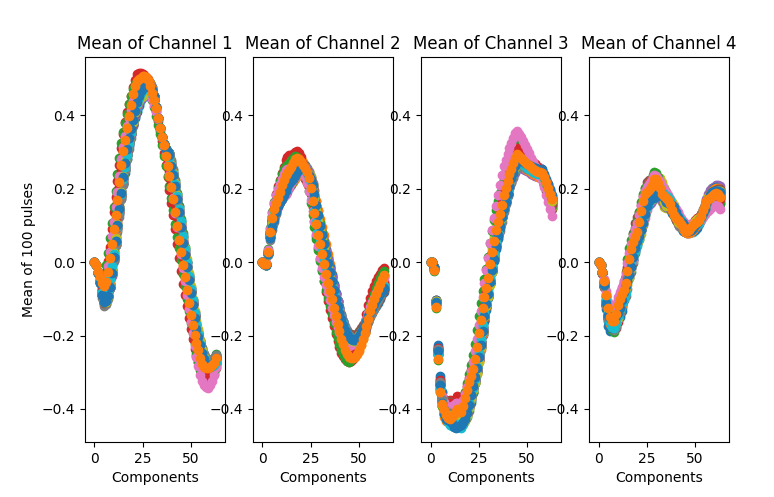
\includegraphics[width=\linewidth]{images/plasticcase}
	\caption{Mean of each channel measured for the plastic case}
	\label{fig:plasticcase}
\end{figure}

In the binary dataset, the minimum and maximum components observed all followed a similiar shape as the average, but the book class did contain one severe outlier in two plots. The full plots are included in the submission under \url{plots/binarybook.png} and \url{plots/binaryplasticcase}, in which the plot of the minimum components in channel one and the maximum components in channel three both include one row of outliers. Since the average did not deviate from other components for that class, it seemed fair to say that these maximum and minimum readings were outliers. Instead of removing them and risking producing a biased model, the row was left in the data set. The existence of these outliers were noted when choosing a cost function however to try and minimise their affect.



\subsection{Distributions}

\subsection{Relationships}

\section{Feature Selection}

\section{Model Selection and Training}

Since each dataset contains an equal number of samples for each classes, the probability of a random classifier guessing correctly is equal to $$\frac{1}{\textit{Number of Classes}}$$. 

\subsection{Model 1}
\subsection{Model 2}
\section{Evaluation and Comparison}
\section{Discussion}

\bibliographystyle{unsrt}
\bibliography{mybib}

\end{document}
